\documentclass[tikz,border=10pt]{standalone}
\begin{document}
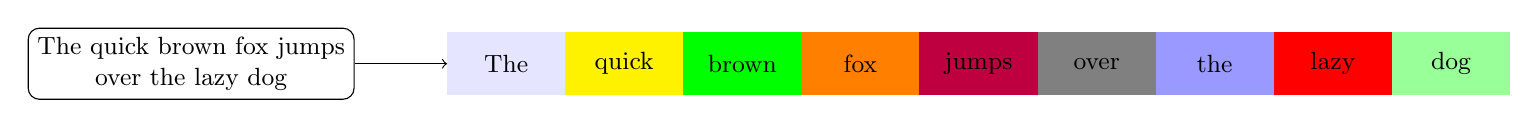
\begin{tikzpicture}[align=center, font=\small]

% Input
\node[draw, rounded corners] (text) at (0, 0) {The quick brown fox jumps\\ over the lazy dog};

% Tokens
\node[fill={blue!10}, minimum width=1.5cm, minimum height=0.8cm] (token) at (4,0) {The};
\node[fill={yellow}, minimum width=1.5cm, minimum height=0.8cm] at (5.5,0) { quick};
\node[fill={green}, minimum width=1.5cm, minimum height=0.8cm] at (7,0) { brown};
\node[fill={orange}, minimum width=1.5cm, minimum height=0.8cm] at (8.5,0) { fox};
\node[fill={purple}, minimum width=1.5cm, minimum height=0.8cm] at (10,0) { jumps};
\node[fill={gray}, minimum width=1.5cm, minimum height=0.8cm] at (11.5,0) { over};
\node[fill={blue!40}, minimum width=1.5cm, minimum height=0.8cm] at (13,0) { the};
\node[fill={red}, minimum width=1.5cm, minimum height=0.8cm] at (14.5,0) { lazy};
\node[fill={green!40}, minimum width=1.5cm, minimum height=0.8cm] at (16,0) { dog};

% Arrow
\draw[->] (text) -- (3.25,0);

\end{tikzpicture}
\end{document}